%%
%%
%%			CHAPTER 4: DESIGN
%%
%%

\chapter{Design} \label{Chapter4}

To meet the research objectives outlined in \textit{Chapter 3}, the requirements defined in \textit{Section \ref{ProposedWork}} must be addressed in the design of the proposed system. With these in mind, an initial system design was devised. 

There are countless factors that must be taken into consideration when designing a research environment, and particularly when a flawed design can have far-reaching implications and consequences for the security of others unaware of the project in the first place. In order to develop solutions that were both secure and effective, every aspect of the design required scrutiny and careful planning. 


\textit{Section \ref{FunctionalConsiderations}} details the \textit{initial} design decisions that were made to address the functional requirements of the research environment.

\textit{Section \ref{DesignChallenges}} addresses a number of identified challenges that required additional analysis to fully satisfy the requirements of the proposed system.

\textit{Section\ref{DesignSummary}} provides a summary, recognising in particular the unpredictable nature of research as it evolves. 

\section{Functional Considerations} \label{FunctionalConsiderations}
This section describes many of the functional design considerations and decisions made relating to the implementation of the research environment. These include initial design decisions regarding the environment deployment platforms, the configuration of the honeynet and the design of the monitoring system.

\subsection{Deployment Platform}
Selection of the hosting infrastructure and platforms for the proposed system was an important consideration in the design which would have a significant impact on the successful development of cyber-incident monitor as well as on the design proposal for adaptive honeypots.

\subsubsection{Choice of Hosting Solution}
%% Should talk about the considerations of hosting it on a local machine (cost, isolation from personal networks and devices a consideration)
The benefits of outsourcing the hosting of services to a third-party cloud platform were discussed at length in {\textit{Section \ref{IaaS}}.} As explained by Vasilomanolakis \textit{et al.}, ''cloud services provide resilience and uptime reliability ... which ensures uninterrupted monitoring.'' \cite{Vasilomanolakis}

Amazon Web Services (AWS) is a subsidiary of Amazon Inc., which describes itself as ''a secure cloud services platform, offering compute power, database storage, content delivery and other functionality to help businesses scale and grow.'' \cite{WhatIsAWS}
        
The AWS Elastic Compute Cloud (EC2) service is a very flexible means of quickly setting up configurable server instances on-demand. Though other hosting solutions including DigitalOcean and Trinity College's OpenNebula infrastructures were considered, the flexibility of options offered by AWS as well as the fact that it is an industry leader in providing cloud services resulted in it ultimately being the hosting platform of choice for this research.

\subsubsection{Use of Containers}
%% In Problem Formulation, should already have identified the fact that it would be most sensible to use containers. This doesn't need to be explained again here, but the reasons for choosing Docker should be.

After first deciding that containers were the platform of choice for deploying honeypots in the proposed system, it was decided that Docker container technology would be used to implement the research environment. Docker is the industry standard for container solutions and is an open-source technology with a global support community.

Some of the benefits of using of Docker containers in particular for the implementation of the research environment include:
\begin{itemize}
\item The fact that each container has an independent networking stack, simplifying the implementation of a honeynet compared to virtual networks or bare-metal.
\item The independence and flexibility of isolated container storage.
\item Docker repositories, the use of which means that a rigorously-audited base OS image can be used as a foundation for the honeypot containers and then built upon with customised configuration options.
\item The existence of research regarding the security of Docker technology. \cite{ExperimentingWithDocker} 
\item The presence of comprehensive documentation for the Docker ecosystem as well as a globally active support community. 
\end{itemize}

All of these factors would enable confident decisions to be made regarding the use of Docker in a security application.

\subsubsection{Host Operating System}
It was decided that Linux-based operating systems would be used for both the EC2 VM hosts and the container images used in the research environment, for a number of reasons.

\begin{enumerate}
\item Linux is regarded to be the most commonly deployed operating system for servers and embedded devices\footnote{Though it is not possible to determine the exact number, in the research conducted by Yinn Min Pa Pa \textit{et al.} it was measured that 91\% of hosts found to be scanning the darknet were running Linux. \cite{IoTPot2016}}.  Targeting the solution at deployment in Linux-based infrastructures is thus most likely to be the real deployment scenario for such a system.
\item Linux is natively supported by almost all open-source and industry tools, which would enable the use of almost any technology in the implementation of the project.
\item It is widely accepted that as a very popular OS for powerful servers, a very large proportion of cyber attacks are targeted at Linux-based systems.
\end{enumerate}
% In particular, Linux-based systems are very common in embedded devices such as those compromised by IoT botnets, making it an obvious choice for this research.
%
\subsubsection{Choice of Honeypot}
Motivated by the level of activity of IoT botnets, it was decided that an IoT honeypot was the most appropriate choice for this project. The Cowrie honeypot, which was discussed in detail in \textit{Section \ref{AboutCowrie}}, is a mature open-source IoT honeypot. It was identified as an ideal option for targeting IoT botnets in the proposed deployment, particularly since it is an SSH/telnet honeypot: The two protocols which have been found to be most highly targeted by recent IoT botnets. \cite{UnderstandingTheMiraiBotnet} \cite{HajimeMysteriousBotnet}

The fact that Cowrie is medium-interaction means that the risks of compromising a real system are mitigated whilst also enabling a relatively high level of interactivity with an attacker. As an open-source project it is also highly configurable, both offering a high degree of customisability and the ability to extend the source code. This is important in order to successfully conduct experiments with a view to proposing effective design approaches for IoT honeypots.

Crucially, Cowrie allows for a high level of interactivity with attackers, whilst also mitigating the risks of compromising a real system such as not providing the ability to execute code but instead storing the SHA-checksum of any attempted downloads. The fact that it is being actively maintained and supported, and that the rudiments of a containerised solution for the honeypot are already in place, are all selling points for the use of the Cowrie honeypot in this research.
        
        %%JSON logging also a benefit: Easy to use it with visualisation tools that are JSON-based such as Elasticsearch.

        
\subsubsection{Container Capabilities}
		It is clearly important to consider how restricted the capabilities of honeypot containers should be in order to capture attacks, whilst also keeping the systems secure. Since the Cowrie honeypot will be running in these containers, if an attacker managed to circumvent the Cowrie application they should be restricted in what activities they can engage in when interacting directly with the underlying container. Additionally, if an attacker was to discover they were being monitored by a honeypot, it is plausible they could launch an attack on the platform on which it is hosted. As quoted from Upi Tamminen a.k.a. \textit{desaster}, the original developer of the Kippo honeypot, ''By running kippo, you're virtually mooning the attackers. Just like in real life, doing something like that, you better know really well how to defend yourself!'' \cite{DesasterQuoteKippo} 
        
        These considerations are addressed more fully in an exploration of the security considerations of using Docker in \textit{Section \ref{DesignChallenges}}. However, overall precautionary measures identified regarding restricting container capabilities include:
        
        \begin{itemize}
        \item Running the honeypot containers as a non-root user, restricting the default privilege level of the containers.
        \item Installation of a minimal quantity of Linux utilities such that an attacker who manages to interface directly with the container will have very few tools at their disposal.
        \end{itemize}
		
        
\subsubsection{Honeynet Design}

As part of the design of the honeynet, a component that provides the functionality of a \textit{honeywall gateway} as described in \textit{Section \ref{HoneynetsExplanationSoA}} is required. This device is the first component of the honeynet that an attacker will interact with, and so should be maximally attractive as a gateway router which if compromised, promises the attacker the compromise of many more devices. % All of the devices could then capture attack data under consistent experimental conditions, allowing for accurate comparisons to be made regarding relative attractiveness.

In order to develop an effective solution using a honeynet, the final design should incorporate measures to meet a number of requirements.

\begin{itemize}
\item It should be simple to configure and maintain control of each component of the honeynet independently.
\item Honeypots in the honeynet should be isolated from the host system as much as possible.
\item It should be easy to scale the honeynet on-the-fly by adding or removing honeypots.
\item The configuration of the honeynet should be portable such that it is straight-forward to remove and redeploy the honeynet environment.
\item It should be possible for an attacker interacting with the honeywall component to map out the configuration of the remainder of the honeypots in the honeynet, facilitating attack propagation and the capture of valuable attack data. It should not however be possible to detect that the system is a honeynet.
\end{itemize}

It was well-understood that deploying and configuring a network of honeypots to meet all of these requirements would be an error-prone and time-consuming process, particularly given limited prior experience with the Linux networking stack. 

Given that it had already been decided to host the project on an AWS EC2 VM instance, hereafter referred to as the \textit{honeypot instance}, this instance would need to be dedicated to hosting multiple containers, inter-networked to appear as though they are individual machines within the same network. The idea of a \textit{honeywall} discussed in Lance Spitzner's 2003 paper \cite{Spitzner:2003:HCI:956415.956438} is clearly a component of major interest in the implementation of the honeynet: This component must be capable of being used as a \textit{jumpbox}\footnote{A jump-box is a term commonly used in networking to refer to a dedicated device on a network that is used to manage devices in a separate security zone.} with outbound network connection capabilities in order to give an attacker access to the rest of the honeynet.

%Also need to be able to evaluate against a baseline implementation: A control is required for the experiments. 
% Maybe this is more appropriate to discuss later, but I think it is important to have thought about during the design (which I did).

      
 \subsubsection{Ease of Deployment} \label{EaseOfDeploymentDesignDecision}
		
		As outlined in \textit{Section \ref{Objective1}}, in order for a honeypot-based system to be feasible to use in a production environment it is key that it is easy to deploy and maintain. In particular, if a honeypot becomes compromised in an attack it should be simple to remove and redeploy it in the system whilst also persisting any data captured by the removed honeypot. Containers have been identified as providing many of these required functions.
        
        One of the significant benefits of container technologies is the ease with which identically configured environments can be deployed. However, the same ease of deployment for a fully-networked system is not something that can be catered for by container technologies. This made it important that a deployment mechanism for the entire system be developed such that it could be removed and reinstated in minimal time.
        
        The identified approach to achieving this was to capture the configuration of the system in a set of bash scripts, which could be used to automate the deployment of the entire honeynet environment. These scripts could be maintained and updated as the configuration of the system evolved, such that if the system was removed it could be identically redeployed using the scripts. These scripts should also include some simple usability measures such as a \textit{usage} function\footnote{Such a function, when specified as a parameter to the script, will typically list the arguments and execution options that are available from that script.} to assist in the efficient and simple deployment of the system.
        
\subsection{Incident Monitoring} \label{IncidentMonitoringDesign}
The incident monitoring component of the proposed system would handle the aggregation, processing and visualisation of data as well as the generation of threat detection alerts. A number of decisions needed to be made regarding how best to achieve this, as explained in the following subsections.

\subsubsection{Isolating the Monitoring System} \label{IsolatingMonitoringSystem}
It is clearly crucial to ensure that the monitoring system which an administrator will rely on for key threat information is minimally susceptible to compromise. Given that the proposed honeypot-driven system is actually intended to invite attacks, this becomes an even more important consideration.

It was decided on this basis that physically isolating the monitoring system as much as possible from the honeypot system would reduce the likelihood of such an event occurring. Hosting the monitoring system on an independent remote EC2 instance would deliver some of this isolation, and so was included as part of the system design. This component is hereafter referred to as the \textit{management instance}. This brings some questions regarding obscuring communication between the honeypot instance and the remote monitoring system into the picture, since it is undesirable for an attacker to notice regular communications between one of their victims and another valuable device. 

\subsubsection{Secure Transfer of Honeypot Logs} \label{SecureLogTransfer}
As data that an attacker would not want captured in relation to their activities, it should not be possible for an attacker to view or to redirect the logs generated by the honeypots to another destination when they are being transported between the honeypots and the monitoring system. Thus, the mechanism for transferring logs between the honeypot instance and the management instance needed to be able to support both origin/destination authentication as well as confidentiality and integrity.


Filebeat is a widely used open-source log-shipping agent which transports log files from client servers to another host. This is exactly the kind of functionality that is required to send the logs generated by the honeypots from the honeypot instance to the management instance. As a technology that is widely supported and used, Filebeat seemed an obvious choice for transporting the log files in the research environment. 

Importantly, with Filebeat it is possible to add the required layer of security by generating an SSL certificate and key pair for the management server. The certificate can then be shared with the honeypot instance, ensuring that Filebeat sends encrypted data only to the trusted management server and vice-versa. \cite{FilebeatSSLProtection}

\subsubsection{Visualisation of Honeypot Log Data} \label{VisualisationDesignChoice}
Visualisation is clearly a key component of the proposed cyber-incident monitor, enabling greater usability and informational value through succinct description of attack data captured by the honeypots. 

The ELK stack is a well-established means of log analysis, aggregation and visualisation. Based on its successful use in the TPot development \cite{TPotWebpagev17} and the fact that it has been endorsed as a visualisation approach for the Cowrie honeypot, \cite{CowrieWebsite} it was decided that the ELK log management stack would be used to process and visualise log data generated by the honeypots\footnote{Though alternative visualisation tools such as Splunk used by the MHN project were also explored, \cite{ModernHoneyNetworkLaunchAnnouncement} the ELK stack was generally found to be less complex and so was the favoured option.}. The Filebeat application discussed in \textit{Section \ref{SecureLogTransfer}} above is also coincidentally developed by the same group, meaning that the interoperability of these tools should be straight-forward to achieve.



%The ELK stack is widely used for visualisation of log data, and in particular is used by the developers of Deutsche Telekom's \textit{TPot} incident monitoring solution.
 
\subsubsection{Intrusion Alert/Notification Mechanism} \label{DesignChoicePSAD}
PSAD is an open-source intrusion detection tool that is used to detect port scans and other malicious traffic on Linux systems. It operates by monitoring the networking logs of the device, and from this determining whether a scan or attack event has occurred. 

PSAD was identified as being a suitable alert mechanism for the purposes of the cyber-incident monitor, since by examining the networking logs of the honeypot instance email notifications could be configured to be sent to a specific email address upon noticing suspicious activity. This would enable timely notification of undesirable activity in a production environment so that remedial action can be taken as soon as possible.

Prior to this, another alerting mechanism built by the same group as the ELK Stack and Filebeat was considered as a potential notification option. The XPack plugin is capable of generating notifications based on the logs received by the ELK stack. \cite{Xpack} However, after consideration it was realised that this would mean that an alert would only be sent to an administrator after the honeypot logs had been processed by the management instance, meaning that there was potential for an unbounded delay in time-to-notification\footnote{It is possible that in an unreliable network, logs generated by the honeypots that contain crucial attack information may be delayed in reaching the management server, meaning that crucial time would be wasted before an alert can be sent to a system administrator. In this time, it is possible that the attacker could have compromised the entire system, rendering this option infeasible.}. This realisation motivated the decision to use PSAD, which would generate the notification as soon as suspicious activity was identified.

%It was also decided that an intrusion alert mechanism such as \textit{Tripwire/Snort/Suricata} could be investigated if there was more time towards the end of the project. However, for a proof-of-concept model the use of PSAD was more than sufficient. % Note that Snort is actually used as part of PSAD.
		


%
% 		SECTION 2: DESIGN CHALLENGES
%


	\section{Challenges} \label{DesignChallenges}
    Additional to the functional design considerations and decisions outlined in the previous section, a number of specific challenges to the implementation of the proposed system were encountered. These were carefully explored and resolved as part of the design of the system.
    
    \subsection{Fingerprinting Honeypot Environments} \label{ChallengeHoneypotFingerprinting}
    As highlighted in \textit{Section \ref{HoneypotSoAChallenges}}, the fingerprinting of honeypot environments by attackers presents an ongoing challenge for honeypot designers. 
        
As was discussed by Barron \textit{et al.} in their study of attacker behaviours using the Cowrie honeypot, it is likely that an informed attacker would be able to fingerprint the Cowrie honeypot as not being a legitimate environment and disconnect. \cite{PickyAttackers2017} For example, by default the Cowrie honeypot assigns hostname \textit{svr04} to the honeypot. An attacker interacting with this honeypot who is aware of the default properties of Cowrie will certainly be aware of this default value and detect that they are interacting with a Cowrie honeypot.

However, in order to conduct a fair comparison between the impact of differently configured characteristics of honeypots in the experiments in this research, it was important to have a plain, out-of-the-box Cowrie installation in the honeynet as a control. Thus it was concluded that in spite of fingerprinting concerns, in each experiment iteration there would need to be one such Cowrie honeypot deployed in the honeynet.
    
    	\subsection{Ethics of Honeypots} \label{EthicsOfHoneypots}
		There are a number of potential ethical issues associated with a project using honeypots that have already been outlined in \textit{Section \ref{HoneypotSoAChallenges}}. A further ethical concern is the ability for a honeypot to be compromised, and then used as an attack platform to launch attacks on other devices. 
  
It is difficult to balance obtaining useful results from research with the inherent risks of implementing a honeypot. This consideration required careful deliberation, after which the following conclusions have been drawn. 	
		
		\begin{itemize}
		\item This risk can safely be viewed as the general risk associated with using devices connected to the web, and not necessarily related to the use of honeypots in particular. This view is in line with that held by Nawrocki \textit{et al.}, who discuss the issue in a survey on honeypot software. \cite{Nawrocki2016}
		
		\item Although it is never possible to entirely eradicate the risk of attack propagation, the honeypot components of the project should be implemented so that they provide mitigation against this risk. The containers in which the Cowrie honeypots would be hosted would be heavily based on the official \textit{Docker-Cowrie} Docker image\footnote{The version of the Docker-Cowrie image off which the images in this research were based was that of January 29th 2017.} \cite{DockerCowrie} developed and endorsed by the maintainers of the Cowrie development community. This container image runs the Cowrie honeypot under a non-root user account with minimal services available within the container, so that even if an attacker did bypass the Cowrie application and gain direct access to the container it is unlikely that they would be able to launch any attacks on other devices.
            
			\item Dedicated research environments where honeypots are isolated from important devices and networks are also effective for protecting external systems. The fact that AWS instances are being used to host the research environment means that the system is being hosted in an environment with enterprise-level security. Given this fact, it is highly unlikely that an attack would have the ability to do any significant damage if it did propagate outside of the system.
		\end{itemize}		
	

    
    	\subsection{Persisting Volatile Container Content} \label{PersistingDockerContent}
        A characteristic of Docker containers is that by default, their contents are not persisted once they stop running: As explained by the developers of the TPot project,  ''all data in docker is volatile. Once a docker container crashes, all data produced within its environment is gone and a fresh instance is restarted.'' \cite{TPotWebpagev16} This is a design feature of containers: As well as enabling a container to be run without any affinity to a specific host, by separating the file system of a container from that of its host it is possible to achieve enhanced security through isolation. 

         In this system, the persistence of logs generated by honeypots running inside these containers is crucial. The solution to this data volatility issue, according to the TPot developers, is to have ''persistent storage ... on the host in order to make (the data) available and persistent across container or system restarts.'' \cite{TPotWebpagev16} This can be achieved through the use of \textit{Docker volumes}, a persistence mechanism available for container directories. Docker volumes are the recommended approach to persisting data that is generated and used by Docker containers. When a container accesses a volume, Docker's storage driver is bypassed and the container interacts directly with the mounted volume on the host file system. 
         
         It was decided that given these considerations, Docker volumes should be used to persist the log data generated by the honeypot containers in the research environment.
         
        
    	\subsection{Docker Security Considerations} \label{DockerSecurityConsiderations}
        As with any technology, there are security concerns about Docker. Though Docker Inc. have a historically excellent record for keeping on top of security of containers and providing extensive documentation, \cite{DockerSecurityDocumentation} there are inherent risks in using containers that have been highlighted in literaure. \cite{7742298} \cite{ExperimentingWithDocker} \cite{LXCsForDeceptiveHoneypots2017} \cite{Chelladhurai2016} \cite{Pisarcik:2014:FDV:2659651.2659685} These have been very carefully contemplated during the undertaking of the project.
   
The greatest security concern identified regarding the use of Docker containers is the potential for an attacker to propagate the attack to the system hosting the containers: Compromise of this system is highly undesirable.

\begin{itemize}
\item Inherently, Docker containers share the kernel of the host, and many claim that this increases the attack surface of Docker containers when compared to VMs: As described by Chelladhurai \textit{et al.}, VMs are only able to communicate with the VM kernel, and not with the host. \cite{Chelladhurai2016} This is a concern that is also raised by Kedrowitsch \textit{et al.} and Pisarcik \textit{et al.} in their use of containers for deploying honeypots. \cite{LXCsForDeceptiveHoneypots2017} \cite{Pisarcik:2014:FDV:2659651.2659685}
\item As described in \textit{Section \ref{PersistingDockerContent}}, a number of Docker volumes are being used to mount directories on the host system to each container. This presents a potential security risk, since an attacker inside a honeypot container could potentially interface directly with the linked host volume and place whatever they want into the mapped directory.
\item The Docker engine is known to automatically create a number of virtual networks on the host on which it is running, so that containers can communicate with the host and with each other. Any connectivity between containers and their host is a risk to the host, since it could potentially result in an attacker connecting into the host machine over a Docker network and compromising a real server.
\end{itemize}

These concerns are not insubstantial, and required careful consideration to handle correctly. The result is a number of reasonable precautionary measures to be incorporated into the initial design as follows:

\begin{itemize}
	\item The isolation characteristic described in \textit{Section \ref{SecurityThroughContainerisation}} in relation to containers addresses the concerns regarding the increased attack surface of containers compared to VMs. Since each container runs in its own namespace and uses its own network stack, provided that careful consideration is given to the shared resources to which it has access and to the privilege level allocated to the container it is possible to sandbox the container quite well from the host machine. This is discussed at length in the Docker security documentation. \cite{DockerSecurityDocumentation}
	\item All honeypot containers to be used in the research should be configured to run the bare minimum of services required to facilitate attacks. This is another measure designed to ensure that the activities of an attacker inside a container are relatively limited.
	\item The containers to be used in the implementation of the honeynet should be built upon well-maintained base OS images from the official Docker Hub repositories. \cite{DockerHub} This will ensure that the most recent security updates available for the base images are inherited by all containers as a robust security foundation.
	\item An effective measure identified by Chelladhurai \textit{et al.} \cite{Chelladhurai2016} is to restrict the networking capabilities of containers as much as possible, allowing communication only between trusted containers. To facilitate this, careful attention needs to be given to the configuration of the containers such that they do not expose any unnecessary ports or belong to any unnecessary networks.
\end{itemize}


\subsection{Enticing IoT Botnet Attacks}
Clearly in order to attract the attention of IoT botnets, identified as the target of choice for the honeynet deployment, the honeypots should be as attractive as possible based on the characteristics of devices that have been found to attract IoT botnets. \cite{UnderstandingTheMiraiBotnet} \cite{BrickerBotArticle} \cite{HajimeMysteriousBotnet} In their paper, the developers of IoTPot discuss the importance of (i) supporting all options that attackers want to use, (ii) providing realistic login interfaces and (iii) facilitating logins, in the successful design of an IoT honeypot. \cite{IoTPot2016}

Upon analysis of related publications and research, a number of IoT device characteristics which are likely to attract IoT botnets were identified as follows:
\begin{itemize}
\item The ability to use brute-force authentication to access a device, i.e. weak or default device credentials.
\item The presence of either or both of the SSH and telnet protocols on the device.
\item An unpatched or vulnerable version of either services present on the device, or of the OS.
\item The presence of ''interesting'' network traffic to or from the IoT device, particularly if that traffic is not encrypted, similar to what was implemented by Dowling \textit{et al.} \cite{Dowling2017}
\item The ability to fingerprint the device as a product of a particular vendor whose devices are widely known to be vulnerable.
\end{itemize}

These characteristics could all be considered as potential variables in the experiments to be conducted, assisting in the proposal of an effective, adaptive design for honeypots targeting IoT botnets.


\subsection{Identifying Attacks from IoT Botnets}
A further difficulty in evaluating any results captured by the honeynet is that of how attacks by human attackers can be distinguished from automated attacks by bots. This distinction is particularly important towards the second objective of the research, where a proposal for designing effective honeypots targeted at IoT botnet attacks is desired.

In a paper detailing observations about attacker behaviours elicited through the use of a large deployment\footnote{The experiments conducted by Barron \textit{et al.} included 102 individual Cowrie honeypots.} of Cowrie honeypots, Barron \textit{et al.} note that ''bots perform specific environment-agnostic actions... human attackers are affected by the underlying environment, e.g., executing more commands on honeypots with realistic files and folder structures''. \cite{PickyAttackers2017} Some of their more specific conclusions are that:

\begin{itemize}
\item Humans care about user files with realistic looking names and data, whereas bots do not;
\item Humans make spelling mistakes when using a shell, whereas bots do not;
\item Bots will behave in the same way regardless of the host that they are running on (i.e. environment agnostic);
\item The time taken between subsequent commands is greater for a human attacker than for a bot, whose sequence of attack commands is automated;
\item Most attackers are bots.
\end{itemize}

These observations are useful in distinguishing human attackers from bots. In order to distinguish IoT botnets from other botnets, observations from literature regarding active IoT botnets offer the most value in discriminating between IoT bots and other bots. \cite{UnderstandingTheMiraiBotnet} \cite{HajimeMysteriousBotnet} For example, both the Mirai and Hajime IoT botnets are known to test for the presence of the BusyBox shell\footnote{BusyBox is a lightweight shell which combines miniature versions of common UNIX utilities into a single
small executable, making it very popular for use in IoT devices.} on victim devices. \cite{Busybox} This test is conducted in order to verify that the device is running a real Linux shell: As explained by Edwards \textit{et al.} in a paper discussing the Hajime IoT botnet, \cite{HajimeMysteriousBotnet} ''a proprietary CLI is likely to reject the command, but a legitimate Linux shell would execute Busybox ... letting Hajime know that it has a bona fide Linux shell''. These kinds of indicators that can be observed through examining logged attack sessions will also aid in identifying the type of botnet behind any attacks captured by the honeynet.


\subsection{Credible Evaluation of Honeypot Experiments}
As already highlighted in \textit{Section \ref{BenefitsForUsingHoneynetForExperiments}}, the use of a honeynet in the proposed research environment enables credible evaluation of the relative performance of different characteristics of honeypots. The design of such an experimental setup however requires that there as few variables between honeypots as possible. Thus, in the honeynet it is necessary to include:
\begin{itemize}
\item A plain, baseline ''control'' device with no enhancements, as discussed in \textit{Section \ref{ChallengeHoneypotFingerprinting}};
\item A variety of improved honeypots, each exhibiting a different variation of the same potentially attractive characteristic. 
\end{itemize}

Taking this approach means that for the purposes of evaluation, the sources of variability in the experiment are maximally controlled: All honeypots will be exposed to attack under the same environmental conditions, with a single controlled variation per honeypot. This approach eliminates the need to account for many otherwise significant environmental variables, such as if the honeypots were each evaluated independently on different host servers. Such variables could otherwise bring the credibility of claims about relative effectiveness of different honeypot characteristics into question.



\section{Summary} \label{DesignSummary}
It was recognised from the beginning that given the unpredictability of research, and in particular the unpredictability of attacks, the requirements of the system and the resulting design were likely to evolve as the project progressed. However, a solid, robust and considered design based on informed decisions, and supported by previous research and current best practice, are sure to contribute positively to the effective implementation of the overall solution.

\begin{figure}[ht]
      \centering
      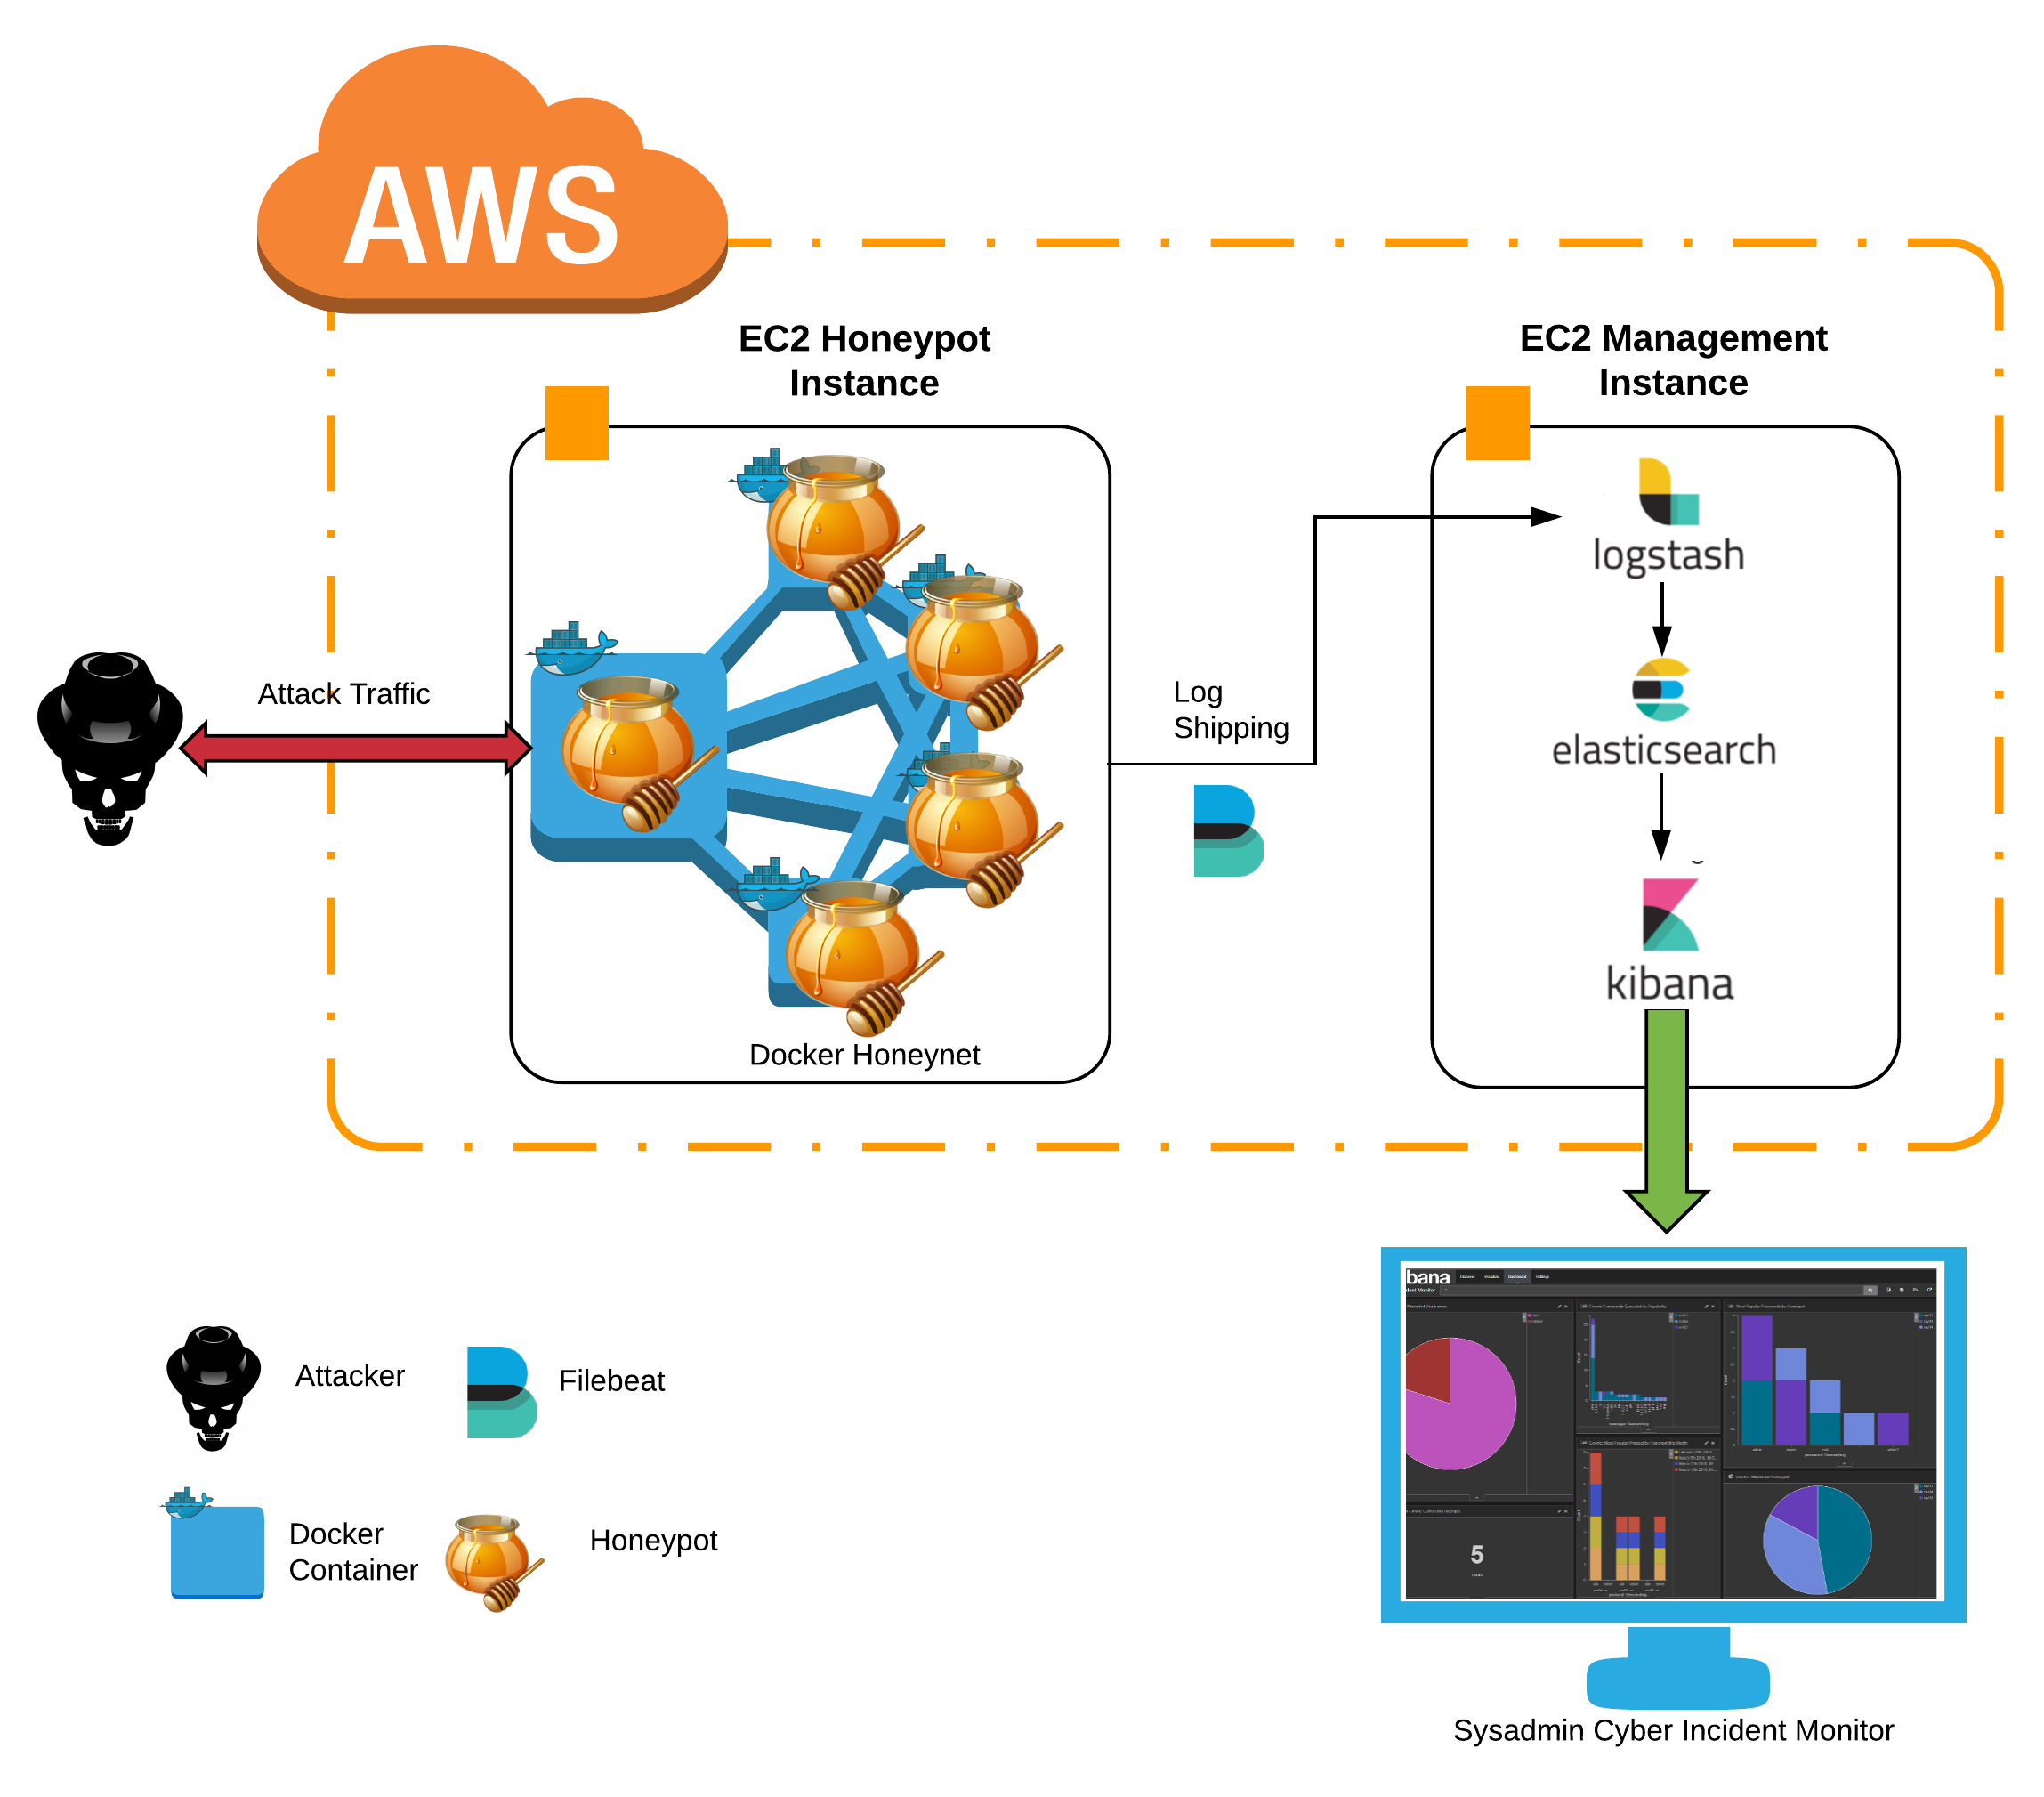
\includegraphics[width=160mm, scale=1]{Images/Cyber_Incident_Monitor_Architecture_Original_Design.png}
      \caption{Overview of the Proposed System Design} 
      \medskip
	  \small
		A high-level overview of the intended architecture and components of the system. The components include 2 AWS EC2 servers, a container network consisting of containerised honeypots hosted on the EC2 honeypot instance, an ELK log processing and visualisation pipeline hosted on the EC2 management instance, and a web console access to the visualisations generated by the system.
\label{fig:CyberIncidentMonitorSystemOriginalDesign}
\end{figure}

%\includewidefigure{CyberIncidentMonitorSystemOriginalDesign}{Overview of the Proposed System Design}{A high-level overview of the intended architecture and components of the system. The components include 2 AWS EC2 servers, a container network consisting of containerised honeypots hosted on the EC2 honeypot instance, an ELK log processing and visualisation pipeline hosted on the EC2 management instance, and a web console access to the visualisations generated by the system.}{Images/Cyber_Incident_Monitor_Architecture_Original_Design.png}

As part of a research progress update for this system 3 months after it had begun, a conceptual diagram similar to that provided in figure ~\ref{fig:CyberIncidentMonitorSystemOriginalDesign} was produced to give a high-level overview of the system architecture and operations. 


